\section{Introduction}


Estimating the burden of the effect of the COVID-19 pandemic on mortality is an important challenge~\citep{weinberger2020estimation}. The estimates of COVID-19 related deaths are subject to testing capacity and changes in definition and reporting guidelines, raising accuracy and completeness considerations \citep{aburto2021estimating, konstantinoudis2021regional}. In addition, the estimates of COVID-19-related deaths give an incomplete picture of the mortality burden of the COVID-19 pandemic, as they do not account for the indirect pandemic effects due to, for instance, disruption to health services~\citep{kaczorowski2021beyond}. Alternatively, excess mortality has been extensively used to evaluate the impact of the COVID-19 pandemic on mortality \citep{rossen2020excess, islam2021excess, kontis2020magnitude, konstantinoudis2021regional, VerbeeckLMMCOVID}.

Excess mortality is estimated by comparing the observed number of deaths in a particular time period with the expected number of deaths under the counterfactual scenario of the event (pandemic) not having had occurred. Typically, this counterfactual scenario is calculated using a comparison period, for instance, several previous years (\url{https://www.euromomo.eu/}). Calculating the expected number of deaths accurately requires accounting for factors such as population trends, seasonality, temperature, public holidays and spatio-temporal dependencies. While accounting for the above-mentioned factors, most studies to date have estimated excess mortality at the national level \citep[see][]{rossen2020excess, weinberger2020estimation}, and some have examined excess mortality across countries~\citep{islam2021excess, kontis2020magnitude, kontis2021lessons}. 

While national-level estimates of excess mortality give valuable insights into the total number of excess deaths, they do not allow for evaluation of within-country geographical differences. However, such information is essential to understand the country's transmission patterns and effectiveness of local policies and measures to contain the pandemic \citep{kontopantelis2021excess}. Temporal trends in excess mortality can substantially differ across regions of the same country \citep{Blangiardo2020}, which makes national-based comparisons even more challenging. Therefore, understanding the effect of the COVID-19 pandemic on mortality requires higher spatial resolution and models that account for spatial, temporal and spatio-temporal dependencies. 

When working at high spatio-temporal resolution, data are generally sparse, and this leads to highly variable excess mortality estimates. This is aggravated by the fact that excess deaths tend to be subject to spatial and temporal correlation. This makes it essential to use statistical methods that can account for these dependencies and provide robust and accurate estimates. The disease mapping framework, which is commonly employed in epidemiology to study the spatio-temporal variation of diseases \citep{waller1997hierarchical, moragarjournal}, can be exploited to estimate excess mortality at subnational and weekly level. The Bayesian approach is naturally suited in this context, as it is able to model complex dependency structures, as well as to incorporate uncertainty in the data generating and modelling process. In addition, while fully propagating the uncertainty, it allows for summaries of results at any desired level of spatio-temporal aggregation (using for instance coarser geographical units suitable for policy implementation). This in combination with fast approximate methods to inference, such as the Integrated Laplace Approximation (INLA; \citealp{rue2009approximate}), make this framework particularly powerful and appealing for the monitoring of the pandemic burden and timely policy making.

Here, we describe how to run a study on excess mortality at high spatial and temporal resolution using a Bayesian approach and R. This tutorial provides a detailed explanation of the modelling approach used previously to quantify excess mortality in 5 European regions \citep{konstantinoudis2021regional}. We have further modified the way we model long-term trends in \citet{konstantinoudis2021regional}, as we showed that it provides more accurate predictions \citep{riou2023direct}. Figure \ref{fig:workflow} illustrates the workflow followed in this paper together with the main R packages used. Source code for replicating the data wrangling (R scripts prefixed with 01, 02 or 03), analysis (R scripts prefixed with 04) and post-processing steps (R scripts prefixed with 05 or 06 and the App folder) and data files are available from GitHub at \url{https://github.com/gkonstantinoudis/TutorialExcess}.\\
\begin{figure}[t]
	\centering
	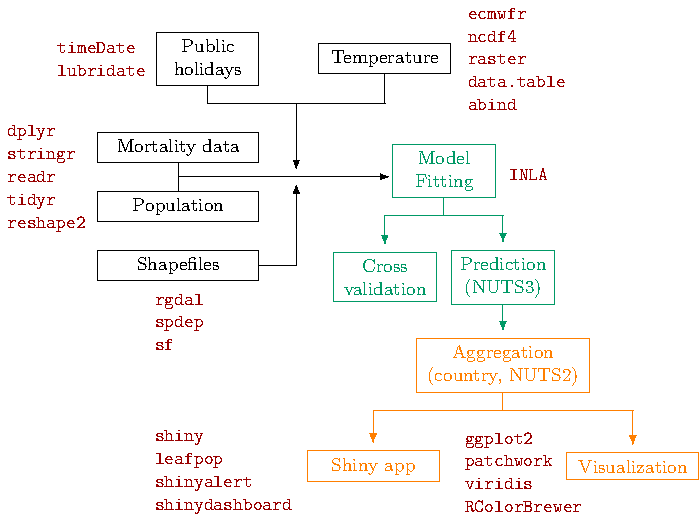
\includegraphics{Workflow.pdf}
	\caption{Diagram of the workflow: data wrangling in black, analysis in green, post-processing in orange and packages in red (timeDate; \citealp{timeDate}, lubridate; \citealp{lubridate}, dplyr; \citealp{dplyr}, stringr; \citealp{stringr}, readr; \citealp{readr}, tidyr; \citealp{tidyr}, reshape2; \citealp{reshape2}, rgdal; \citealp{rgdal}, spdep; \citealp{spdep}, sf; \citealp{sf}, shiny; \citealp{shiny}, leafpop; \citealp{leafpop}, shinyalert; \citealp{shinyalert}, shinydashboard; \citealp{shinydashboard}, ecwmfr; \citealp{ecwmfr}, ncdf4; \citealp{ncdf4}, raster; \citet{raster}, data.table; \citealp{data.table}, abind; \citealp{abind}, ggplot2; \citealp{ggplot2}, patchwork; \citealp{patchwork}, viridis; \citealp{viridis}, RColorBrewer; \citealp{RColorBrewer}). NUTS stands for Nomenclature of Territorial Units for Statistics with NUTS3 being the highest spatial resolution available and NUTS2 coarser but appropriate for policy making.}
	\label{fig:workflow}
\end{figure}
This tutorial is structured as follows: we first describe the modelling framework and present the case study in Italy. We then show how to run and evaluate the model, and extract and visualise the results. Finally, we present an R-shiny app which makes the results effectively and easily disseminated. 




\section{Bayesian hierarchical spatio-temporal model to estimate excess mortality}


We propose a Bayesian hierarchical model to quantify the effect of spatio-temporal location on excess mortality under extreme events such as the COVID-19 pandemic, stratified by specific age-sex population groups. To do so, we first describe the statistical model for predicting the number of deaths from all-causes based on historical data, in the counterfactual scenario in which the pandemic did not take place. Then, we show how to estimate the magnitude of excess deaths over a specific period of time, with associated uncertainty, by comparing the predicted versus the actual number of deaths.

Let $y_{jstk}$ and $P_{jstk}$ be the number of all-cause deaths and the population at risk for the $j$-th week, $j=1, \dots, J_t$, where $J_t$ is the total number of weeks of the year $t$ ($t=2015, \dots 2019$), the $s$-th spatial unit ($s=1, \dots S$, where $S$ is the number of provinces in Italy), and $k$-th age-sex group ($k = 1, \dots 10$). Also let $x_{1jt}$, $x_{2t}$ and $z_{jst}$ denote the adjustment covariates, respectively: public holidays ($x_{1jt}$ = 1 if week $j$ of the $t$-th year contains a public holiday and 0 otherwise), the year that the $j$-the week belongs to, and temperature. We assume that the historical observed number of deaths, conditional on the risk $r_{jstk}$, follows a Poisson distribution, with a log-linear model for the risk. To simplify notation, we omit $k$, although the following model was fitted to all $k$ age-sex groups (with the elements of the linear predictor also depending on $k$):

\begin{align} \label{eq:1}
\begin{split}
y_{jst}|r_{jst} \sim & \text{Poisson}\big(\mu_{jst}=r_{jst}P_{jst}\big),  \\
\log \left(r_{jst} \right) & = \beta_{0jt} + \beta_{1} x_{1jt} + \beta_{2} x_{2t} + f(z_{jst}) + b_{s} + w_{jt}.
\end{split}
\end{align}

Here, $\beta_{0jt}$ is the week-specific intercept in year $t$ given by $\beta_{0jt}=\beta_{0}+\epsilon_{jt}$ for the $k$-th age-sex group, where $\beta_{0}$ is the global intercept and $\epsilon_{jt}$ is an unstructured random effect representing the deviation of each week from the global intercept, which is modelled using independent and identically (iid) distributed Gaussian prior distribution with zero-mean and variance equal to $\tau_\epsilon^{-1}$. The parameters $\beta_1$ and $\beta_2$ are  unknown regression coefficients associated to the public holidays covariate $x_{1jt}$ and a long term linear trend. The effect of temperature, $f(\cdot)$, is allowed to be non-linear by specifying  a second-order random walk (RW2) model:

\begin{equation*}
z_{jst} \mid z_{(j-1)st}, z_{(j-2)st}, \tau_z \sim \text{Normal}\left(2z_{(j-1)st}+z_{(j-2)st},\tau_z^{-1}\right),
\end{equation*}

\noindent where $\tau_z^{-1}$ is the variance.

Terms $b_s$ and $w_j$ are spatial and temporal random effects, respectively. We specify the spatial random effect term, $b_s$, with a convolution prior \citep{besag1991bayesian}, and the temporal random effect term, $w_j$ with a non-stationary in time prior. In detail, we model $\boldsymbol{b}$ using a reparameterisation of the popular Besag-York-Molli\'e prior, which is a convolution of an intrinsic conditional autoregressive (CAR) model and an iid Gaussian model. Let $u_s$ be the spatially structured component defined by an intrinsic CAR \citep{Besag1974} prior  $u_s|u_i,i\in \partial_s \sim(\bar{u},\tau_u^{-1}/m_s)$, where $\bar{u}$ is the mean of the neighbours and $\partial_s$ and $m_s$ are respectively the set and the number of neighbours of area $s$,  $\tau_u^{-1}$ the conditional variance, and $v_s$  the unstructured component with prior $v_s \overset{iid}{\sim} \text{Normal}(0,\tau_v^{-1})$. We model $b_s$ as follows \citep{besag1991bayesian, riebler2016intuitive,  konstantinoudis_discrete}:
\[
b_s=\frac{1}{\sqrt{\tau_b}}\left(\sqrt{1-\phi}v^\star_s+\sqrt{\phi}u^\star_s\right)
\]
where $u_s^\star$ and $v_s^\star$ are standardised versions of $u_s$ and $v_s$ such that their variance is equal to 1 \citep{simpson2017penalising}.
The term $0\leq \phi\leq 1$ is a mixing parameter, which measures the proportion of the marginal variance explained by the structured effect.
Finally, we assign to the temporal random effect term, $w_{jt}$, a Gaussian random walk model of order 1 (RW1). This component captures seasonality and is specified as:
\[
w_{jt} \mid w_{(j-1)t}, \tau_w \sim \text{Normal}(w_{(j-1)t},\tau_w^{-1}).
\]

The Bayesian representation of the above model is completed once we select priors for the fixed effects $\beta_0$ and {\boldmath$\beta$} and the hyperparameters: $\tau_{\epsilon}, \tau_z, \tau_b, \tau_w,$ and $\phi$. For the fixed effects we selected minimally informative Normal distributions, whereas for the hyperparameters we specified "penalising complexity" (PC)  priors \citep{simpson2017penalising}. PC priors are defined by penalising deviations from a ``base'' model (e.g.,~specified in terms of a specific value of the hyperparameters) and have the effect of regularising inference, while not implying too strong prior information. Technically, PC priors imply an exponential distribution on a function of the Kullback–Leibler divergence between the base model and an alternative model in which the relevant parameter is unrestricted. This translates to a suitable ``minimally informative'', regularising prior on the natural scale of the parameter.

In order to quantify the weekly excess mortality at sub-national level for specific age-sex population groups, we need to predict the number of deaths that would be expected if the COVID-19 pandemic had not occurred. In Bayesian analysis, this can be performed by drawing random samples from the posterior predictive distribution (that is, the distribution of unobserved values conditional on the observed values from previous years). Specifically, letting $\pmb{\theta}$ be the model parameters, $\mathcal{D}$ be the observed data, and $y_{jst^{*}}$ be the count of deaths that we want to predict, we have:

\begin{equation}\label{eq:2}
p(y_{jst^{*}}\mid \mathcal{D}) = \int p(y_{jst^{*}}\mid\pmb{\theta}) p(\pmb{\theta}\mid\mathcal{D})d\pmb{\theta}.
\end{equation}

Operationally, we first generate random samples from the joint posterior marginal of the parameters specified in Equation (\ref{eq:1}) at the highest spatial resolution available (NUTS3 regions; Nomenclature of Territorial Units for Statistics 3 regions, \url{https://ec.europa.eu/eurostat/web/nuts/background/}). Following that, we use the samples to compute the linear predictor, compute the mean parameter of the Poisson distribution via inverse link function, and obtain the predicted number of deaths, which represents the baseline number of deaths assuming the pandemic did not take place. 

Finally, to estimate the excess deaths, the predicted number of deaths is compared against the actual observed number of deaths. Further, this allows us to compute the relative change in mortality (relative to what we would expect if the pandemic did not occur). This is obtained by (i) subtracting the predicted number of deaths from the observed number of deaths in each time point $j$ in the  $t^*$-th year and spatial unit $s$ (number of excess deaths or NED), and (ii) dividing NED by the predicted number of deaths for each sample and multiplying by 100 (yielding \% relative excess mortality or REM).

The model estimates are computed using Integrated Nested Laplace Approximation (INLA; \citealp{rue2009approximate}, which performs approximate Bayesian inference on the class of latent Gaussian models \citep{rue2005gaussian}. Unlike simulation based Markov chain Monte Carlo method, INLA is a deterministic algorithm, which employs analytical approximations and efficient numerical integration schemes to provide accurate approximations of the posterior distributions in short computing times. The INLA software is provided through the R package \texttt{INLA}, which can be downloaded from \url{https://www.r-inla.org/}. 

\section{Motivating example: Italy}

\subsection{Outcome data}
We retrieved all-cause mortality data during 2015-2020 in Italy from the Italian National Institute of Statistics (\url{https://www.istat.it/}). Data were available weekly (ISO week), by age (5-year age groups), sex and NUTS3 regions. As the COVID-19 mortality rates increase with  age, we aggregated mortality counts based on the following age groups: $<$40, 40-59, 60-69, 70-79 and 80 years and older \citep{davies2021community}. 


\subsection{Population data}
Population data in Italy during 2015-2020 were retrieved from the Italian National Institute of Statistics. The data represent the population in Italy on first of January of every year stratified by age (5-year age groups), sex and NUTS3 regions. To retrieve weekly population, we performed linear interpolation by the selected age groups ($<$40, 40-59, 60-69, 70-79 and 80$+$), sex, and NUTS3 regions using populations on the first of January of the current and next year. Population counts on the first of January 2021, which takes COVID-19 deaths in 2020 into consideration, were available at the time of analysis. Our goal was, however, to predict mortality  for 2020, as if the pandemic had not occurred. Thus we performed an additional linear interpolation by age,  sex and NUTS3 regions to predict the population at January 1st 2021, using the years 2015-2020 (Figure~\ref{fig:popplot}, panel A). Object \texttt{pop} is a \texttt{tibble} containing the NUTS3 region ID (\texttt{NUTS318CD}), age group (\texttt{ageg}), sex (\texttt{sex}), year (\texttt{year}) and population counts (\texttt{population}):

\begin{figure}[!b]
	\centering
	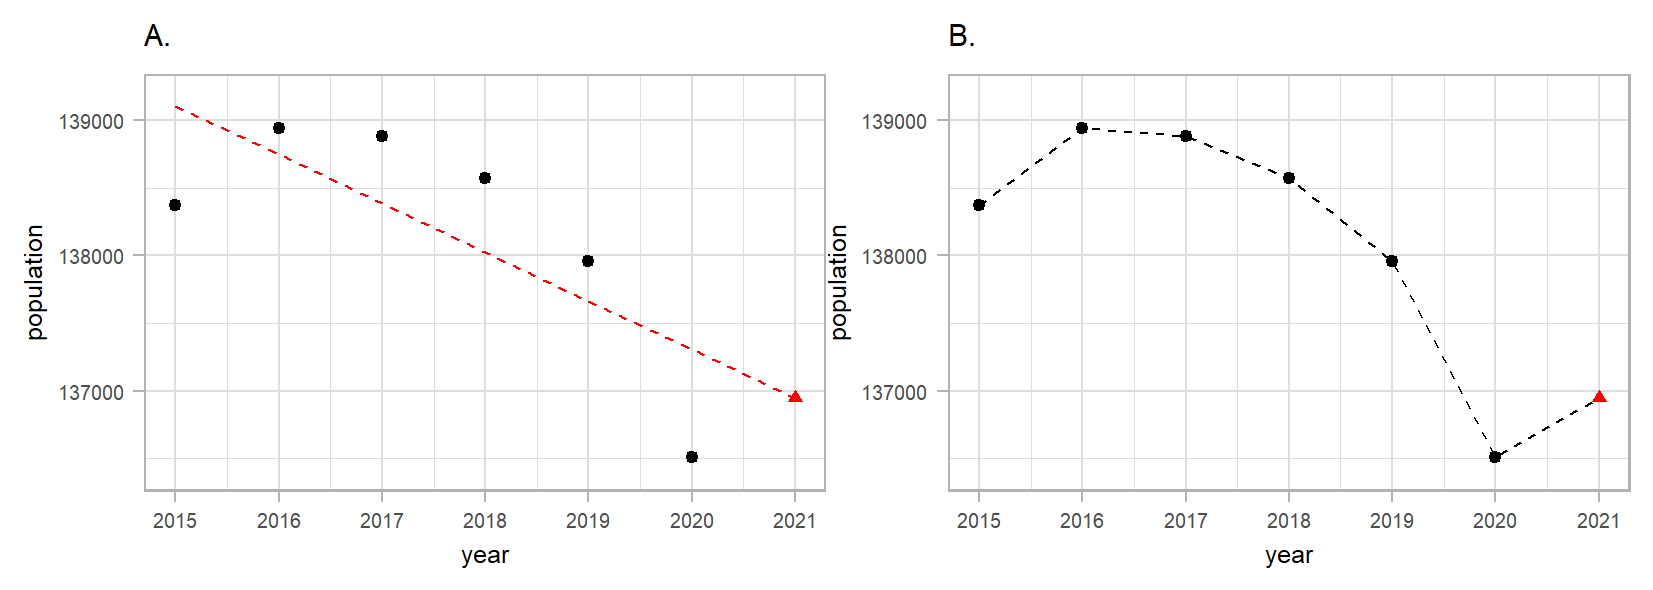
\includegraphics{PopulationPlot.png}
	\caption{A schematic representation of the weekly population estimation procedure focusing on females aged 40-49 in Venice during 2015-2019 as an example. On panel A we show how we used the historical data (black points) and fit a linear regression (red dashed line) to predict 2021 (red triangle). On the panel B we show how we predicted weekly population by drawing lines between the years.}
	\label{fig:popplot}
\end{figure}

\begin{example}
pop
# A tibble: 6,420 x 5
# Groups:   ageg, sex [10]
NUTS318CD ageg   sex     year population
<chr>     <fct>  <chr>  <dbl>      <dbl>
1 TO        less40 female  2015     435758
2 TO        less40 female  2016     427702
3 TO        less40 female  2017     420498
4 TO        less40 female  2018     413141
5 TO        less40 female  2019     406937
6 TO        less40 female  2020     402768
7 TO        less40 male    2015     449605
8 TO        less40 male    2016     443941
9 TO        less40 male    2017     439522
10 TO        less40 male    2018     433365
# ... with 6,410 more rows
\end{example}



We can use the following code (based on \texttt{tidyverse} and "piping" principles) to calculate the population of the 1st of January 2021 by NUTS3 regions, sex and age:
\begin{example}
pop %>% group_by(NUTS3, sex, age) %>% 
	summarise(pop = as.vector(coef(lm(pop ~ year)) %*% c(1, 2021))) %>% 
	mutate(year = 2021) -> pop2021
\end{example}

We acknowledge that the linear trend in the population is a rather simplistic assumption. In subsequent analyses in Switzerland, we proposed a spatio-temporal approach similar with equation (\ref{eq:1}) to model the population counts had the pandemic not occurred \citep{riou2023direct}. The code for that analysis is also online available online (\url{https://github.com/jriou/covid19_ascertain_deaths}).\\
Once we obtained the year 2021 we performed an additional linear interpolation to calculate weekly number of population as shown on Figure~\ref{fig:popplot}, panel B.

\begin{widefigure}[!b]
	\centering
	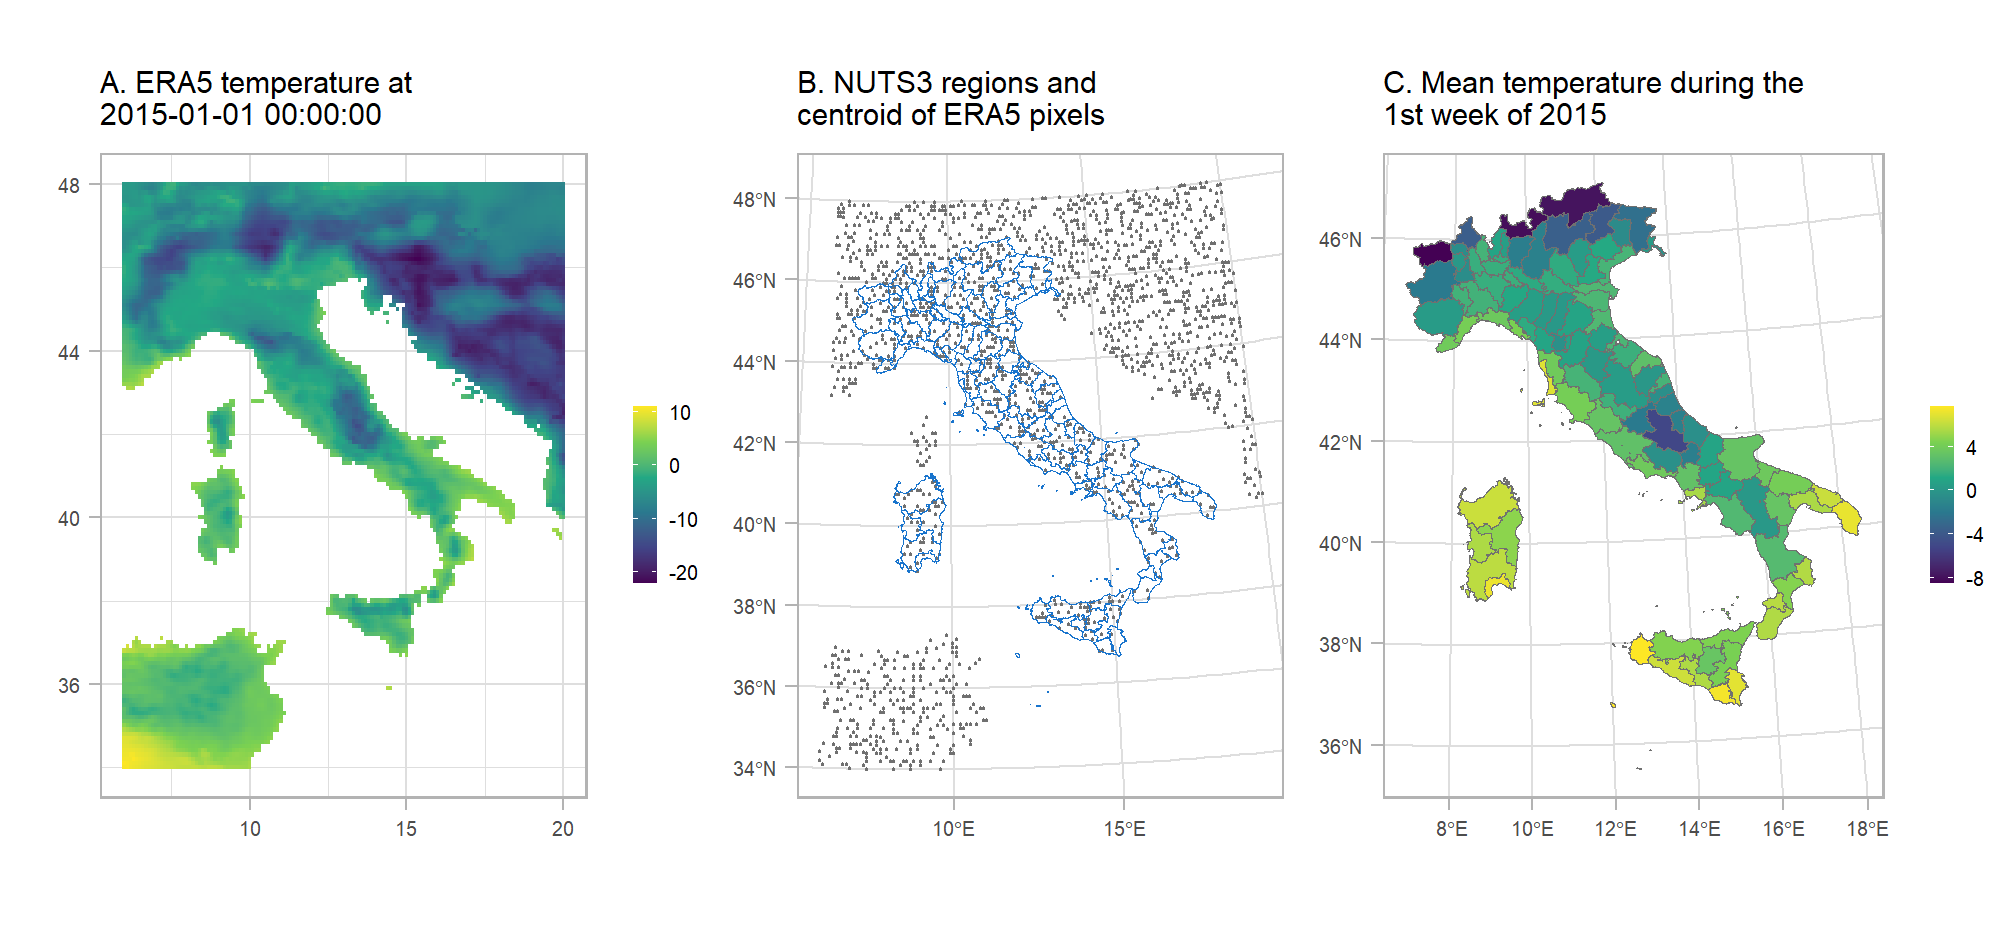
\includegraphics{ERAPOINTS.png}
	\caption{Schematic representation of the temperature misalignment procedure. A) The temperature obtained by ERA5 at 2015-01-01 00:00:00. B) NUTS3 regions in blue and a sample of the centroids of the pixels from the ERA5 raster. C. Mean temperature per NUTS3 region during the 1st week of 2015.}
	\label{ERA5POINTS}
\end{widefigure}

\subsection{Covariates}
We used covariates related to ambient temperature, national holidays, and year of death, to improve the model's predictions. Data on air temperature during 2015-2020 in Italy at 2m above the surface of land were retrieved from the ERA5 reanalysis data set of the Copernicus climate change program \citep{hersbach2020era5}. The geographical resolution of the ERA5 estimates is 0.25$^\circ\times 0.25^\circ$ (panel A of Figure \ref{ERA5POINTS}). We calculated the weekly mean by the centroids of the 0.25$^\circ\times 0.25^\circ$ grid (panel B of Figure \ref{ERA5POINTS}) and then averaged the weekly temperature over the ERA5 centroids that overlay with the NUTS3 regions (panels B and C of Figure \ref{ERA5POINTS}). 


\subsection{Fitting the model}
The modelling process in \texttt{INLA} consists of three main steps: (1)~the selection of priors, (2)~definition of the model "formula" (which sets out the expression for the generalised linear predictor), and (3)~the call to the main function \texttt{inla}, which computes the estimates. 

In particular, we constructed the PC priors for $\sigma_\epsilon=\sqrt{1/\tau_\epsilon}, \sigma_z=\sqrt{1/\tau_z}, \sigma_b=\sqrt{1/\tau_b}$ and $\sigma_w=\sqrt{1/\tau_w}$ based on the assumption that it is unlikely to have a relative risk higher than $\exp(2)$ based solely on spatial, yearly and seasonal variation, Figure~\ref{fig:priors}, panel A. For the mixing parameter $\phi$, we set $\text{Pr}(\phi<0.5) = 0.5$ reflecting our lack of knowledge about whether overdispersion or strong spatial autocorrelation should dominate the field~$b$, Figure~\ref{fig:priors}, panel B.

These assumptions can be encoded using the following code:
\begin{example}
# Defines the priors
hyper.bym <- list(
	theta1 = list('PCprior', c(1, 0.01)), 
	theta2 = list('PCprior', c(0.5, 0.5))
)
hyper.iid <- list(theta = list(prior="pc.prec", param=c(1, 0.01)))

# Defines the model "formula"
formula = 
	deaths ~ 1 + offset(log(population)) + hol + id.year + 
	f(id.tmp, model = 'rw2', hyper = hyper.iid, constr = TRUE, scale.model = TRUE) +
	f(id.wkes, model = 'iid', hyper = hyper.iid, constr = TRUE) + 
	f(id.time, model = 'rw1', hyper = hyper.iid, constr = TRUE, scale.model = TRUE,
	 cyclic = TRUE) +
	f(id.space, model = 'bym2', graph = "W.adj", scale.model = TRUE, constr = TRUE, 
	hyper = hyper.bym)
	
control.family = inla.set.control.family.default()

# Calls INLA to fit the model
inla.mod = inla(formula,
	data = dat,
	family = "Poisson",  
	verbose = TRUE, 
	control.family = control.family,
	control.compute = list(config = TRUE), 
	control.mode = list(restart = T),
	num.threads = round(parallel::detectCores()*.8), 
	control.predictor = list(link = 1))
\end{example}

\begin{figure}[t!]
	\centering
	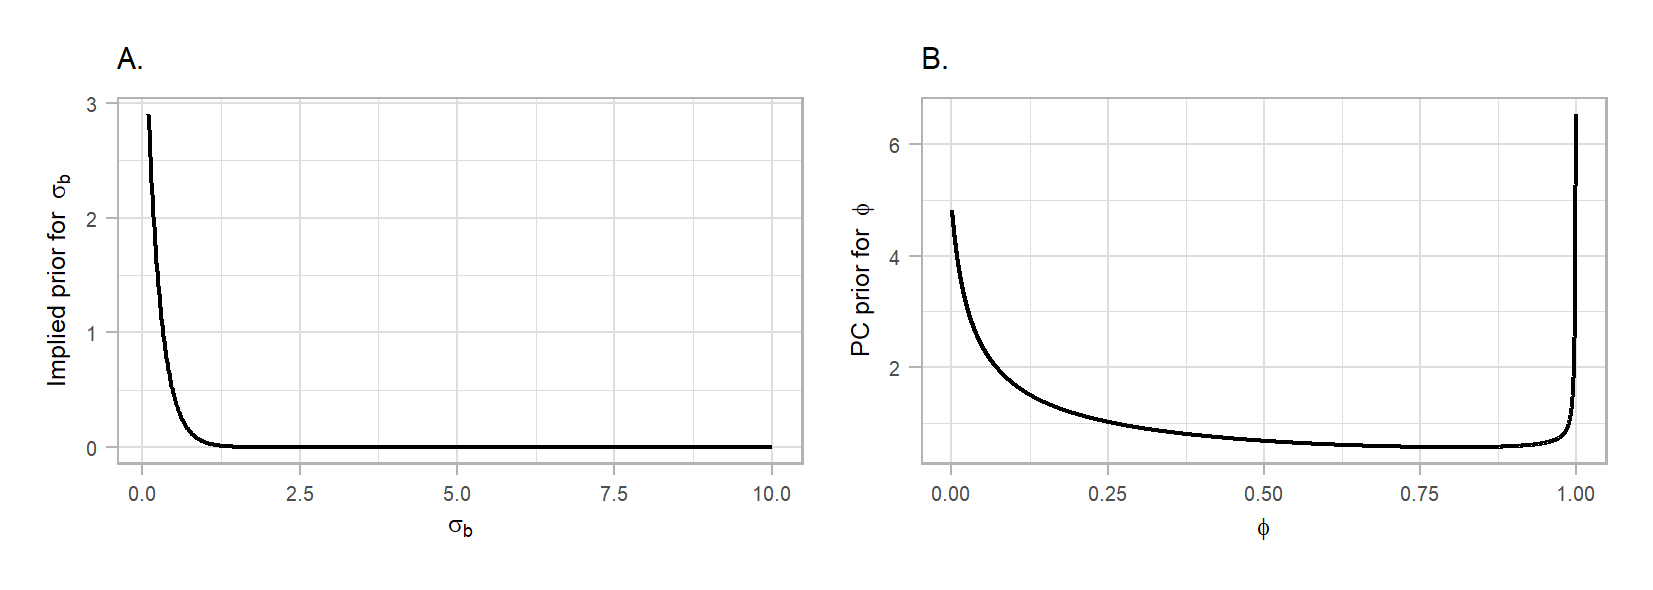
\includegraphics{PCpriors.png}
	\caption{Penalised complexity (PC) priors for the hyperparameters of the spatial field. A) The implied PC prior for the standard deviation (as the original scale of the prior is the precision). B) The PC prior for the mixing parameter $\phi$.}
	\label{fig:priors}
\end{figure}

After fitting the model, we take 1000 samples from the (approximated) posterior distribution of the linear predictor and we use each drawn sample as the mean of a Poisson distribution to retrieve the predicted mortality counts:

\begin{example}
post.samples <- inla.posterior.sample(n = 1000, result = inla.mod)
predlist <- do.call(cbind, lapply(post.samples, function(X)
exp(X$latent[startsWith(rownames(X$latent), "Pred")])))
	
pois.samples <- apply(predlist, 2, function(Z) rpois(n = length(Z), lambda = Z))
\end{example}

This allows us to estimate the entire predictive posterior distribution of the mortality counts, incorporating both the sampling and the linear predictor uncertainty.

\subsection{Model validation}
To examine model validity, we performed a cross validation, leaving out one historical year at a time and predicting the weekly number of deaths by NUTS3 regions for the year left out. As part of this validation we used future years to train predictions for past, but in a previous study we also showed that the model selected was performing well when other types of cross-validations were used \citep{riou2023direct}. For each stratum, we calculated the correlation between observed and fitted and a coverage probability, i.e. the probability that the observed death fall into the 95\% credible interval (95\% CrI) of the predicted. 

\section{Results}
\subsection{Cross-validation}
Overall, we found that the model performed well in predicting the expected number of deaths. The correlation between true and  expected number of deaths varied from 0.39 (95\% CrI: 0.37, 0.40) in females 40$<$ to 0.95 (95\% CrI: 0.94, 0.95) in females  80$>$ and coverage probability from 0.92 in females 40$<$ to 0.96 in males 60-69, 70-79: 
\begin{example}
#              Correlation Coverage
# less40F 0.39 (0.37, 0.40)     0.92
# 40-59F  0.78 (0.77, 0.78)     0.95
# 60-69F  0.83 (0.82, 0.83)     0.95
# 70-79F  0.91 (0.90, 0.91)     0.95
# 80plusF 0.95 (0.94, 0.95)     0.95
# less40M 0.51 (0.50, 0.52)     0.93
# 40-59M  0.83 (0.83, 0.84)     0.95
# 60-69M  0.87 (0.86, 0.87)     0.96
# 70-79M  0.92 (0.91, 0.92)     0.96
# 80plusM 0.94 (0.94, 0.94)     0.95
\end{example}


\subsection{Expected number of deaths}

The object \texttt{pois.samples.list} contains 1000 samples from the posterior predictive distribution (\ref{eq:2}), i.e. 1000 samples of the expected number of deaths by age, sex, NUTS3 regions and week, had the pandemic not occurred. We can access the different age-sex groups as follows:
\begin{example}
names(pois.samples.list)
# "F_less40" "F_40_59"  "F_60_69"  "F_70_79"  "F_80plus" 
# "M_less40" "M_40_59"  "M_60_69"  "M_70_79"  "M_80plus"
\end{example}

\noindent where F stands for females and M for males across the different age groups. To get an idea about the structure of the data, we can use the \texttt{head()} function for females 60-69 and check the first 10 samples (V1 through to V10) of excess deaths for the first 6 weeks of 2020 in the 001 region (Torino)
\begin{example}
pois.samples.list$F_60_69 %>% 
select(paste0("V", 1:10), EURO_LABEL, ID_space, year) %>% 
head()
#     V1 V2 V3 V4 V5 V6 V7 V8 V9 V10 EURO_LABEL ID_space year
# 262 22 18 17 15 17 18 13 19 16  17   2020-W01      001 2020
# 263 18 16 21 20 16 23 13 12 23  17   2020-W02      001 2020
# 264 17 23 20 26 12 16 12 19 17  13   2020-W03      001 2020
# 265 13  8 13 30 22 17 16 22 17  19   2020-W04      001 2020
# 266 14 20 15 15 19 18 23 14 12  18   2020-W05      001 2020
# 267 17 14 14  9 14 15 17 19 19  14   2020-W06      001 2020          
\end{example}
	
\noindent  We can also calculate median and 95\% CrI expected number of deaths for this specific age-sex group across all years by NUTS3 region:
\begin{example}
pois.samples.list$F_60_69 %>% 
select(starts_with("V"), "ID_space") %>% 
	group_by(ID_space) %>% 
	summarise_all(sum) %>% 
	rowwise(ID_space) %>% 
	mutate(median = median(c_across(V1:V1000)), 
LL = quantile(c_across(V1:V1000), probs= 0.025), 
UL = quantile(c_across(V1:V1000), probs= 0.975)) %>% 
	select(ID_space, median, LL, UL) %>% 
	head()
		
# A tibble: 107 × 4
# Rowwise:  ID_space
# ID_space median    LL    UL
# <chr>     <dbl> <dbl> <dbl>
# 1 001         814  748   885.
# 2 002          72   55    90 
# 3 003         139  116   167 
# 4 004         212  183.  243.
# 5 005          86   67   107 
# 6 006         178  150   208 
# 7 007          46   33    62 
# 8 008          86   68   107 
# 9 009         113   93   135.
# 10 010         341  301.  380 
# … with 97 more rows
\end{example}
	
\subsection{Excess mortality}
	
The above results can be combined in different ways using the functions \texttt{get2020data()} and \\ \texttt{get2020weeklydata()} to calculate excess mortality (in the R script functions.R). The function \texttt{get2020data()} aggregates over the entire country, NUTS2 regions, sex, age and time resulting in the object \texttt{d}, whereas the function \texttt{get2020weeklydata()} aggregates over the entire country, NUTS2 regions, sex and age but not over time resulting in the object \texttt{d\_week}.
	
\begin{example}
names(d)
# "province" "region"   "country" 
names(d$province)
# "none"   "age"    "sex"    "agesex"
names(d$province$age)
# "40<"   "40-59" "60-69" "70-79" "80+"  
names(d$province$sex)
# "F" "M"
names(d$province$agesex)
# "F40<"   "F40-59" "F60-69" "F70-79" "F80+"   "M40<"   "M40-59" "M60-69" "M70-79" "M80+" 
\end{example}
		
Province stands for the NUTS3 regions (the resolution we used to fit the models), region for the NUTS2 (coarser than NUTS3, appropriate for policy making) and country for the nationwide aggregation. Within these aggregations users can select the option "none" being the total aggregation by age and sex, "age" by sex, "sex" by age  and "agesex" refers to no age and sex aggregation. The objects \texttt{d} and \texttt{d\_week} have similar structure and contain summary statistics for REM and NED and posterior probabilities of a positive REM or NED: 
		
\begin{example}
head(d$province$none)
# Simple feature collection with 6 features and 24 fields
# Geometry type: POLYGON
# Dimension:     XY
# Bounding box:  xmin: 6.626865 ymin: 44.06028 xmax: 9.21355 ymax: 45.95041
# CRS:           +proj=longlat +datum=WGS84
# ID_space SIGLA     DEN_UTS observed population mean.REM median.REM   sd.REM
# 1      001    TO      Torino    32478  2226317.2 21.37414   21.36545 1.116582
# 2      002    VC    Vercelli     3216   168761.7 32.27082   32.15534 3.133142
# 3      003    NO      Novara     5274   364529.4 23.62994   23.71569 2.220801
# 4      004    CN       Cuneo     8716   585479.3 20.16665   20.22069 1.742638
# 5      005    AT        Asti     3745   211437.1 26.37080   26.30691 2.660622
# 6      006    AL Alessandria     7916   416090.6 28.27706   28.21510 2.052881
# LL.REM   UL.REM exceedance.REM median.REM.cat exceedance.REM.cat median.pred
# 1 19.19396 23.50963              1           20%>          (0.95, 1]       26761
# 2 26.51331 38.74179              1           20%>          (0.95, 1]        2434
# 3 19.18442 27.97865              1           20%>          (0.95, 1]        4263
# 4 16.67966 23.54490              1           20%>          (0.95, 1]        7250
# 5 21.19545 31.77340              1           20%>          (0.95, 1]        2965
# 6 24.48449 32.33309              1           20%>          (0.95, 1]        6174
# LL.pred UL.pred mean.NED median.NED    sd.NED   LL.NED   UL.NED exceedance.NED
# 1   26296   27249 5717.153     5717.5 246.42447 5229.975 6182.075              1
# 2    2318    2543  783.265      782.5  57.49419  673.975  898.025              1
# 3    4121    4428 1006.667     1011.0  76.69947  848.925 1153.000              1
# 4    7055    7471 1461.215     1466.0 105.25269 1245.975 1661.075              1
# 5    2842    3092  780.189      780.0  62.31281  654.950  903.000              1
# 6    5982    6360 1743.404     1742.0  98.74248 1556.975 1934.125              1
# median.NED.cat exceedance.NED.cat                       geometry
# 1          1000>          (0.95, 1] POLYGON ((7.859044 45.59758...
# 2    [500, 1000)          (0.95, 1] POLYGON ((8.204465 45.93567...
# 3          1000>          (0.95, 1] POLYGON ((8.496878 45.83934...
# 4          1000>          (0.95, 1] POLYGON ((7.990897 44.82381...
# 5    [500, 1000)          (0.95, 1] POLYGON ((8.046805 45.12815...
# 6          1000>          (0.95, 1] POLYGON ((8.405489 45.20148...
\end{example}

Notice that the object \texttt{d\$province\$none} is a simple feature collection, making mapping it straight-forward using the \texttt{ggplot2} package and \texttt{geom\_sf} function.
In Figure~\ref{SpatiotemporalRegions} (plots 1A, 2A and 3A) we show the median posterior of REM for total age and sex at the national, NUTS2 and NUTS3 regional level. For these plots we used the object \texttt{d} with the selection "none" and plot the median REM (\texttt{median.REM}), for example for 3A:
\begin{example}
# prov <- "Foggia"
# d$province$none %>% 
#	filter(DEN_UTS == prov) %>% 
#	select(geometry) %>% 
#	ggplot() +  
#		geom_sf(data = d$province$none, aes(fill = median.REM.cat)) + 
#		geom_sf(fill = NA, col = col.highlight, size = .8) + 
#		scale_fill_manual(values=colors, name = "", drop = FALSE) + 
#       theme_light() + ggtitle(paste0("3A. NUTS3 regions: ", prov)) 
\end{example}
			

\noindent Overall, the REM in Italy during 2020 was between 15-20\%, meaning that 15-20\% more people died that year than how many would be expected based on historical data, see Figure~\ref{SpatiotemporalRegions}, panel 1A. When the higher geographical resolution is assessed, it was revealed that north and in particular Lombardia was the region hit the worst, with the REM exceeding $20\%$, see Figure~\ref{SpatiotemporalRegions}, panels 1B and 1C. Figure~\ref{PosteriorProb} shows a measure of uncertainty of the REM, now for the different age groups and both sexes (selection "age"). The probability of a positive excess (\texttt{exceedance.REM}) in older people was larger than 0.95 almost everywhere, see Figure~\ref{PosteriorProb}.
		
Panels 1B and 1C of Figure~\ref{SpatiotemporalRegions} show the median temporal nationwide excess mortality together with 95\% CrI by sex after aggregating the different age groups (using \texttt{d\_week} and the "sex" selection). We observe a clear first pandemic wave during March and May and a second one during mid October and December in 2020. During the first pandemic wave, there were weeks when the median REM reached almost 100\% in males, Figure~\ref{SpatiotemporalRegions}.
		
\begin{widefigure}[H]
	\centering
	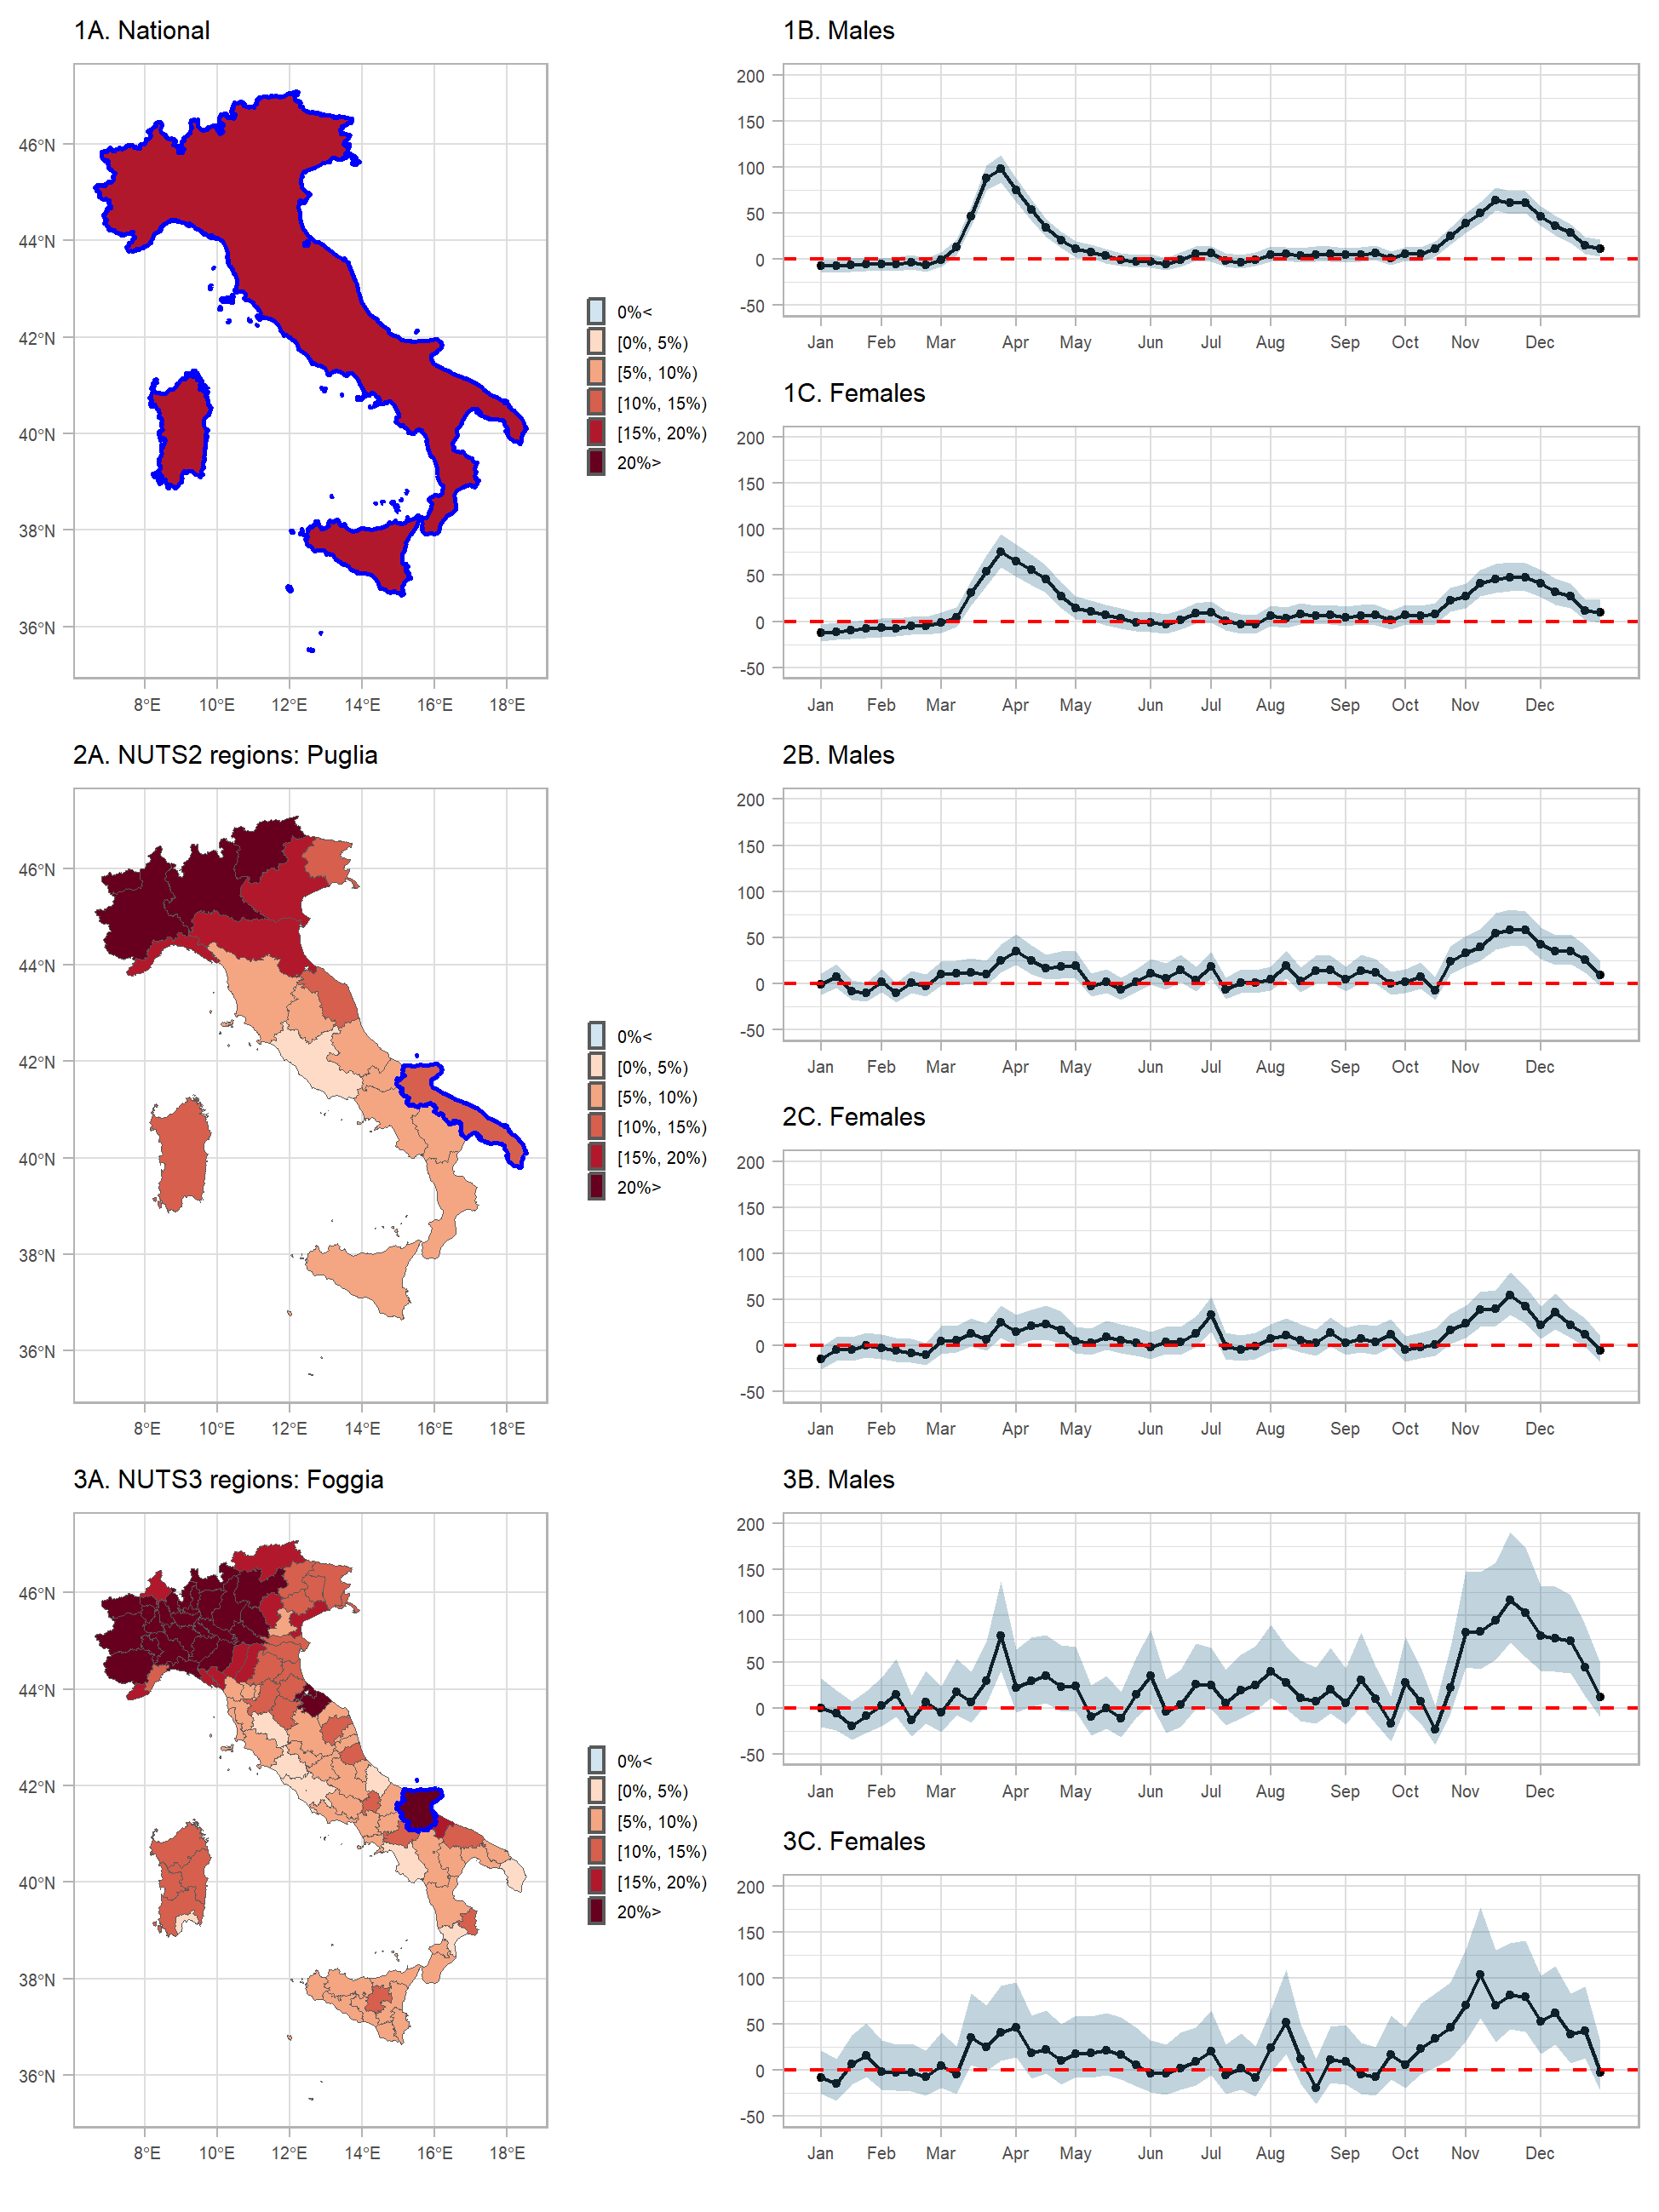
\includegraphics[width=0.92\textwidth]{SpatiotemporalRegions.png}
	\caption{Median relative excess mortality by spatial region during 2020: 1A) nationwide, 2A) NUTS2 and 3A) NUTS3 level, and weekly median relative excess mortality and 95\% credible intervals (95\% probability that the true value lies within this interval) by sex during 2020 in: 1B) males nationwide, 1C) females nationwide, 2B) males in Puglia, 2C) females in Puglia, 3B) males in Foggia and 3C) females in Foggia.}
	\label{SpatiotemporalRegions}
\end{widefigure}	

Panels 2B, 2C, 3B and 3C of Figure~\ref{SpatiotemporalRegions} show the median spatio-temporal excess mortality together with 95\% CrI by sex after aggregating over the different age groups. Panels 2B and 2C highlight the region of Puglia, where during the first wave of the pandemic experienced increases excess mortality. This increase follows similar trends as the nationwide excess mortality (Panels 1B and 1C). When we increase the spatial resolution in panels 3B and 3C, we highlight the province of Foggia, where there was insufficient evidence of a positive excess during the first wave, but strong during the second.

\begin{widefigure}[H]
	\begin{flushright}
		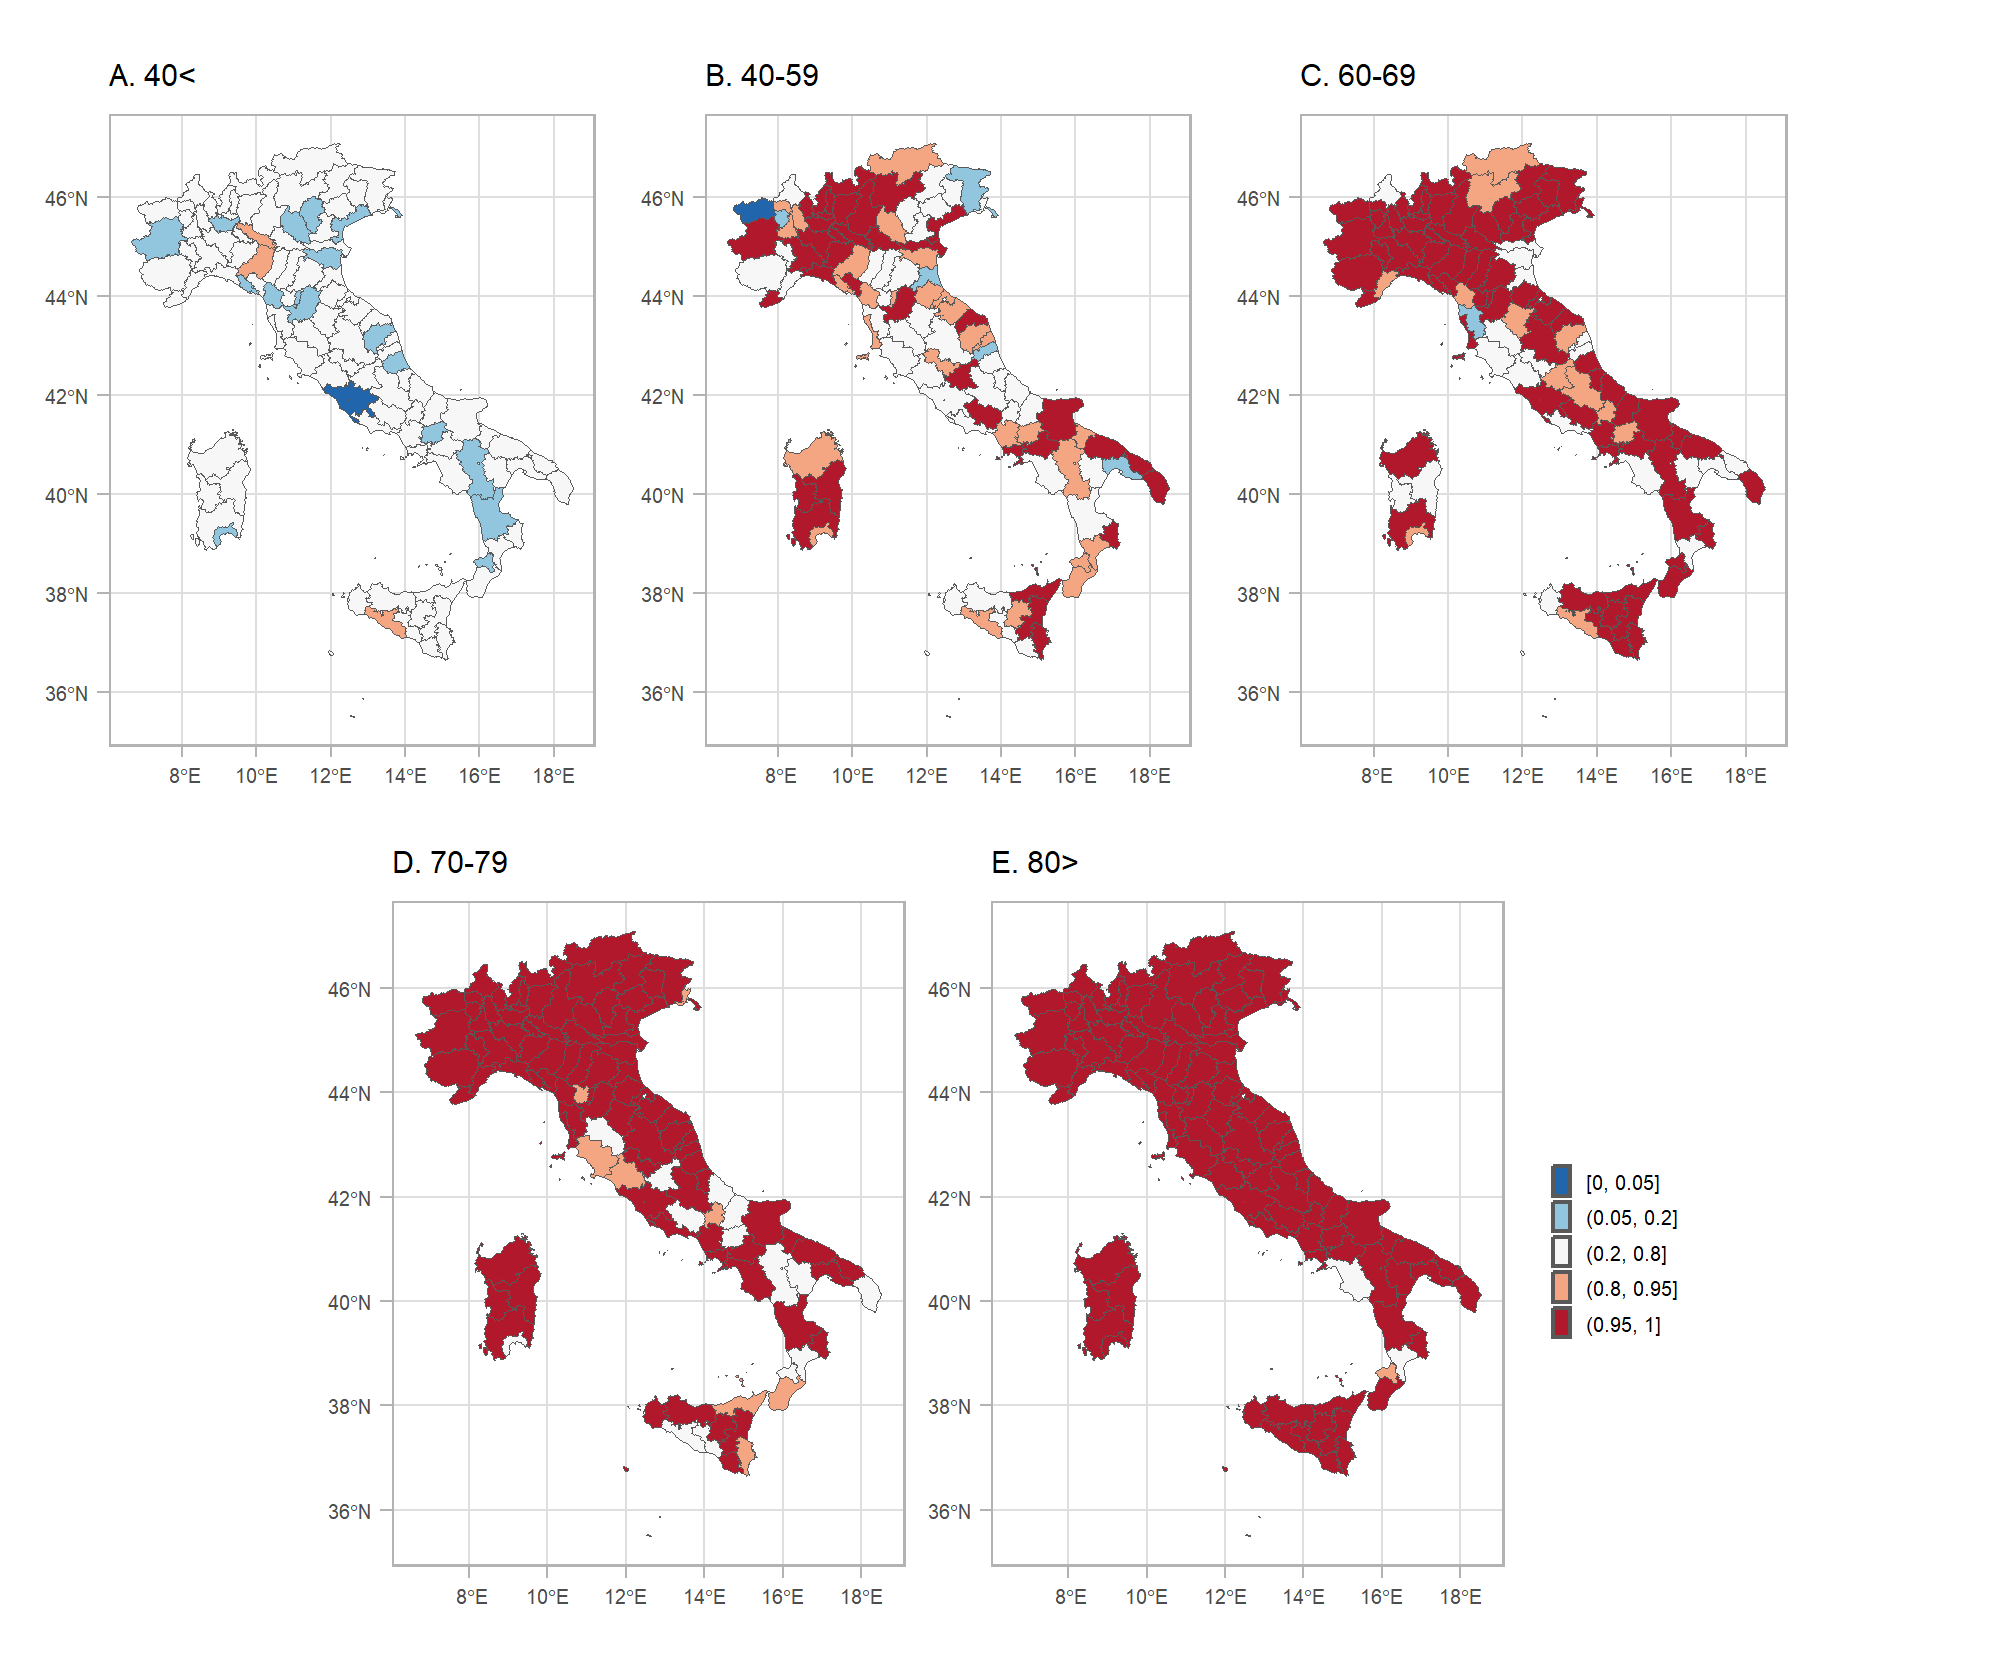
\includegraphics{PosteriorProb.png}
	\end{flushright}
	\caption{Posterior probability that the relative excess mortality is positive for both sexes during 2020 by age group and NUTS3 region. }
	\label{PosteriorProb}
\end{widefigure}
		
\begin{widefigure}[!t]
	\begin{center}
		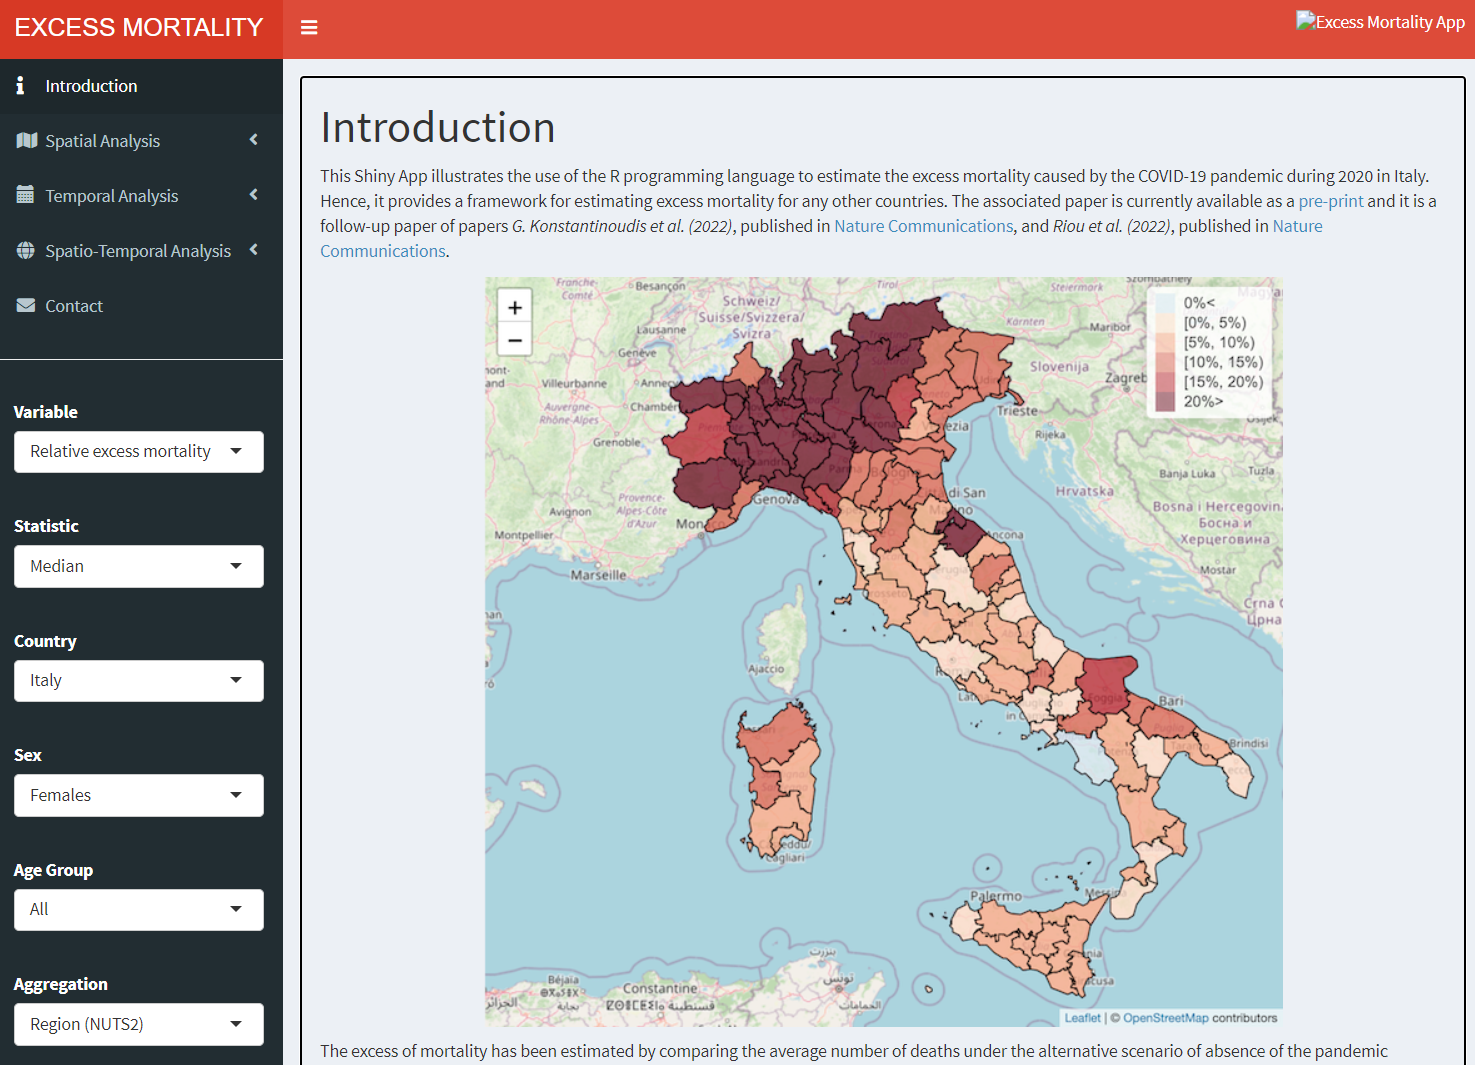
\includegraphics[width=0.9\textwidth]{ShinyApp.png}
	\end{center}
	\caption{Shiny App developed to navigate through the excess mortality estimates during 2020 in Italy across the different aggregations.}
	\label{shinyapp}
\end{widefigure}

\subsection{Shiny Web-Application}
To be able to effectively examine and communicate the different aggregation levels of the output of our modelling framework, we have also developed a Shiny Web-Application (WebApp), Figure~\ref{shinyapp}. The WebApp provides spatial, temporal and spatio-temporal analysis tabs, and within each tab there are plots and summary statistics for the level of aggregation selected from the drop-down menu. Users can select across different variables (REM or NED), statistics (median or posterior probability), sex (males, females or both), age group ($40<$, $40-59$, $60-69$, $70-79$, $80>$ and all) and different geographical level (national, NUTS2 or NUTS3 regions). Summary statistics for each area are available and they are displayed in a pop-up window, which is activated by clicking on the area of interest. In addition, graphical pop-ups are provided to show the weekly estimates for each area with the \texttt{leafpop} \texttt{R}-package \citep{leafpop}, in the spatio-temporal analysis tab. \\
The WebApp that we have developed is hosted at \url{http://atlasmortalidad.uclm.es/italyexcess/}.  
		
\section{Summary}
This tutorial provides a detailed explanation of the workflow used previously to calculate excess mortality during the COVID-19 pandemic in 5 European regions \citep{konstantinoudis2021regional}. The main model used here is slightly modified based on updated results \citep{riou2023direct}. We have proposed a Bayesian workflow for estimating excess mortality and shown how to use \texttt{R} and \texttt{INLA} to retrieve fast and accurate estimates. The proposed workflow also allows for combining different models and presenting the results stratified by age, sex, spatial and temporal location. We have given a practical example of how to use the proposed framework to model the excess mortality during the 2020 COVID-19 pandemic in Italy at small area level. We also developed a Shiny App to effectively communicate the results. The methodological framework can be extended to monitor excess mortality caused by other extreme events; for instance, natural hazards such as tropical cyclones \citep{parks2022association} or heatwaves \citep{konstantinoudis2023bayesian}. Potential methodological extensions of the proposed framework also include modelling the younger age groups with a zero-inflated Poisson distribution. The proposed framework can also be extended to provide an automated tool for online disease surveillance and policy making. 
			
\section*{Acknowledgements}
		
All authors acknowledge infrastructure support for the Department of Epidemiology and Biostatistics provided by the NIHR Imperial Biomedical Research Centre (BRC). The authors also acknowledge infrastructure support for the domain of the shiny app from the University of Castilla-La Mancha.
		
G.K. is supported by an MRC Skills Development Fellowship [MR/T025352/1] and an Imperial College Research Fellowship. M.B. is supported by a National Institutes of Health, grant number [R01HD092580-01A1]. Infrastructure support for this research was provided by the National Institute for Health Research Imperial Biomedical Research Centre (BRC). The work was partly supported by the MRC Centre for Environment and Health, which is funded by the Medical Research Council (MR/S019669/1, 2019-2024). V.G.R. is supported by grant SBPLY/17/180501/000491 and SBPLY/21/180501/000241, funded by Consejer\'ia de Educaci\'on, Cultura y Deportes (JCCM, Spain) and FEDER, and grant PID2019-106341GB-I00, funded by Ministerio de Ciencia e Innovaci\'on (Spain). We thank Univesidad de Castilla-La Mancha for hosting the server on which the Shiny App is running.
		
		
\section*{Author contributions}
		
V.G.R. conceived the study. M.B. supervised the study. G.K. developed the initial study protocol and discussed it with M.B., M.C., M.P. and G.B.. G.K. developed the statistical model, prepared the population and covariate data and led the acquisition of mortality data. M.C. and V.G.R. validated and modified accordingly the code. G.K. ran the analysis. G.K., V.G.R., M.B., M.C. and M.P. wrote the initial draft and all the authors contributed in modifying the paper and critically interpreting the results. V.G.R. developed the Shiny app. All authors read and approved the final version for publication.
		
%\section*{Competing interests}
%The authors declare no competing interests.
		
%\section*{Ethics}
%The study is about secondary, aggregate anonymised data so no additional ethical permission is required.
		
